\documentclass[tikz,border=2pt]{standalone}
\usepackage{amsmath,amssymb}
\usetikzlibrary{arrows.meta}

\begin{document}
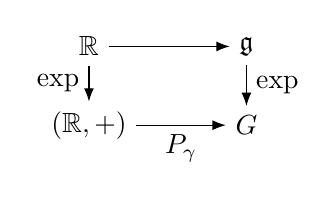
\begin{tikzpicture}[>=Latex,every node/.style={font=\normalsize}]
  \node (A) at (0,1) {$\mathbb{R}$};
  \node (B) at (2,1) {$\mathfrak{g}$};
  \node (C) at (0,0) {$(\mathbb{R},+)$};
  \node (D) at (2,0) {$G$};

  \draw[->] (A) -- (B);
  \draw[->] (A) -- node[left] {$\exp$} (C);
  \draw[->] (B) -- node[right] {$\exp$} (D);
  \draw[->] (C) -- node[below] {$P_\gamma$} (D);
\end{tikzpicture}
\end{document}
